\chapter{Apendix}

\begin{figure}[htpb]
    \centering
    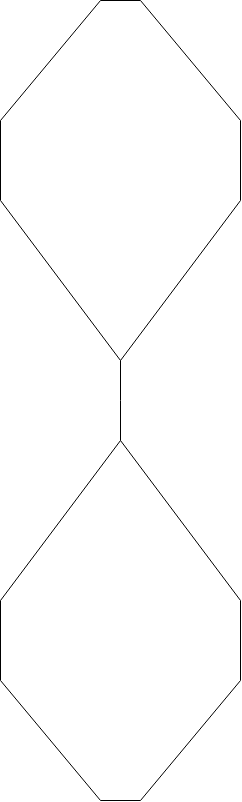
\includegraphics[width=\textwidth]{figures/plots/ballMove}
    \caption{ Schematic for the path of the ball }
    \label{fig:ballMove}
  \end{figure}


\begin{table}[htpb]
    \caption[Ball Directions]{Directions of the Target} \label{tab:ballMove}
    \centering
    \begin{tabular}{|c| c |c|}
        \toprule
        Step & X & Y  \\
        \midrule
          0 &  0.5 & 0.0 \\
          1 &  2.0 & 1.5 \\
          2 &  1.0 & 0.0 \\
          3 &  1.5 & -1.25 \\
          4 &  0.0 & -0.5 \\
          5 &  -1.5 & -1.25 \\
          6 &  -1.0 & 0.0 \\
          7 &  -2.0 & 1.5 \\
          8 &  -2.0 & 1.5 \\
          9 &  -1.0 & 0.0 \\
          10 &  -1.5 & -1.25 \\
          12 &  0.0 & -0.5 \\
          13 &  1.5 & -1.25 \\
          14 &  1.0 & 0.0 \\
          15 &  2.0 & 1.5 \\
          16 &  0.5 & 0.0 \\ 
        \bottomrule
    \end{tabular}
  \end{table}
  